\documentclass[12pt,openany,oneside,a4paper]{scrbook}
%\documentclass[11pt,openany,a4paper,oneside]{scrbook}
%\documentclass[11pt,a4paper,oneside]{scrbook}
\usepackage[left= 2cm,right = 2cm, bottom=2cm, top=2cm]{geometry}
\usepackage{graphicx}
\usepackage[english]{babel}
\usepackage{amsmath}
\usepackage{amssymb}
\usepackage{amsthm}
\usepackage{dsfont}
\usepackage{stmaryrd}

\usepackage{multirow}
\usepackage{booktabs}
\usepackage{hyperref}
\renewcommand{\baselinestretch}{1.15}\normalsize

\usepackage{url}
\usepackage{bm}

\usepackage[T1]{fontenc}
\usepackage[utf8]{inputenc}
\usepackage{float}
\usepackage{multirow}
\usepackage{fancyvrb}
\usepackage{booktabs}
\usepackage{subfigure} 
%MatLab Code
\usepackage[framed,numbered]{matlab-prettifier}
\lstloadlanguages{Matlab}
\usepackage{hyperref}
% Standard Packages
\usepackage{graphicx, subfig}
\usepackage{fancyhdr}
\usepackage[section]{placeins}
%\graphicspath{{img/}}
\usepackage{lmodern}
\usepackage{color}


\definecolor{myred2}{rgb}{1,0.1,0}
\newcommand{\red}{\color{myred2}}

\definecolor{mygray}{rgb}{0.9,0.9,0.9}
\definecolor{darkblue}{rgb}{0.0,0.0,0.6}

\definecolor{myred}{rgb}{0.5, 0.0, 0.13}
\definecolor{pink}{rgb}{0.93, 0.23, 0.51}
% \definecolor{myred}{rgb}{220,20,60}
\definecolor{lugia}{rgb}{0.75,0.75,0.75}
\definecolor{pummelluff}{rgb}{0.8,0.1,0.2}
\newcommand{\com}{\color{lila}}
%\newcommand{\coblass}{\color{grey}}
%\newcommand{\clb}{\color{blue}}
\newcommand{\cob}{\color{myblue}}
\newcommand{\cor}{\color{myred}} 
 % \newcommand{\cor}{\color{red}}
\newcommand{\cog}{\color{gruen}}
\newcommand{\cosi}{\color{lugia}}
\newcommand{\coli}{\color{pummelluff}}

% Umgebungen
\theoremstyle{plain}
%\renewcommand{\baselinestretch}{1.1}\normalsize
\newenvironment{Beweis}{\begin{proof}[\textbf{Beweis}]}{\end{proof}}
\newtheorem{Lemma}{Lemma}[chapter]
\newtheorem{Proposition}[Lemma]{Proposition}

\newtheorem{Corollary}[Lemma]{Corollary}
\newtheorem{Axiom}[Lemma]{Axiom}
\newtheorem{Example}[Lemma]{Example}
\newtheorem{Definition}[Lemma]{Definition}
\newtheorem{Remark}[Lemma]{Remark}

\usepackage{pdfpages}

%\newtheorem{Algorithmus}{\textbf{Algorithmus}}[section]
%\def\Real{{{\rm I\!R}}}
%\usepackage{chngcntr}
%\counterwithin{equation}{chapter}
%
%\usepackage[ruled, algochapter]{algorithm2e}
%\newcommand\mycommfont[1]{\footnotesize\ttfamily\textcolor{purple}{#1}}
%\SetCommentSty{mycommfont}
%\SetAlgorithmName{Algorithmus}{algorithmautorefname}

% Tabellen umfließen lashsen
\usepackage{graphicx}
\usepackage{wrapfig}
%
\usepackage{mathtools,xparse}
\usepackage{tikz}
\usepackage{bigints}
\usetikzlibrary{mindmap}
\usetikzlibrary{positioning}
\usepackage{marvosym}
\usetikzlibrary{svg.path}
\usepackage{todonotes}
\usepackage{arydshln} 


\usepackage{listings}
\lstset{language=C++}
\lstset{
  numbers=none,
  basicstyle=\ttfamily,
  columns=fullflexible,
  %frame=single,
  backgroundcolor = \color{mygray},
  xleftmargin = 0.5cm,
    xrightmargin = 0.5cm,
  showstringspaces=false,
  commentstyle=\color{darkblue}\upshape,
  stringstyle=\color{pink},
  identifierstyle=\color{black},
  keywordstyle=\color{myred},
  morekeywords={xmlns,version,type, name, value,string, vec2D_dbl_Type, vec_dbl_Type, Matrix, AssembleFE_Type}% list your attributes here
}
\renewcommand{\lstlistingname}{Code}

%\usepackage{verbatim}
%
%\usepackage{pgf,tikz,pgfplots}
%\usetikzlibrary{arrows.meta}
%\tikzset{
%  >={Latex[width=1.5mm,length=1.5mm]},
%     base/.style = {rectangle, rounded corners, draw=black,
%                           minimum width=2.5cm, minimum height=1cm,
%                           text left, font=\footnotesize},
%     activityStarts/.style = {base, fill=white!10},
%    class1/.style = {base, minimum width=5.5cm, fill=white!10},
%    class2/.style = {base, minimum width=5.5cm, fill=white!10},
%    class3/.style = {base, minimum width=5.5cm, fill=white!10},
%   	class0/.style = {base, minimum width=3.4cm, minimum height=1.25cm, fill=white!10},
%   	class4/.style = {base, minimum width=3.5cm, minimum height=1.75cm, fill=white!10}
%}

%\pgfplotsset{compat=1.15}
%\usepackage{mathrsfs}
%\usepackage{varwidth}
%\usepackage{enumitem}
% Lade Makros

\begin{document}
% Fraktur Buchstaben
\newcommand{\C}{\ensuremath{\mathbb{C}}}
\newcommand{\R}{\ensuremath{\mathbb{R}}}
\newcommand{\M}{\ensuremath{\mathbb{M}}}
\newcommand{\K}{\ensuremath{\mathbb{K}}}
\newcommand{\Q}{\ensuremath{\mathbb{Q}}}
\newcommand{\Z}{\ensuremath{\mathbb{Z}}}
\newcommand{\N}{\ensuremath{\mathbb{N}}}
\renewcommand{\P}{\ensuremath{\mathbb{P}}}
\newcommand{\E}{\ensuremath{{\mathbb{E}}}}
\renewcommand{\L}{\ensuremath{{\mathbb{L}}}}
%\renewcommand{\bJ}{\ensuremath{{\mathbb{J}}}}
% Script Buchstaben
\newcommand{\cA}{\ensuremath{\mathcal{A}}}
\newcommand{\cP}{\ensuremath{\mathcal{P}}}
\newcommand{\cN}{\ensuremath{\mathcal{N}}}
\newcommand{\cE}{\ensuremath{\mathcal{E}}}

\newcommand{\cO}{\ensuremath{\mathcal{O}}}
\newcommand{\cC}{\ensuremath{\mathcal{C}}}
\newcommand{\cI}{\ensuremath{\mathcal{I}}}
\newcommand{\cS}{\ensuremath{\mathcal{S}}}
\newcommand{\cF}{\ensuremath{\mathcal{F}}}
\newcommand{\cL}{\ensuremath{\mathcal{L}}}
\newcommand{\cT}{\ensuremath{\mathcal{T}}}
\renewcommand{\P}{\ensuremath{\mathcal{P}}}
\renewcommand{\d}{\ensuremath{\text{d}}}


% Integral in Grenzen
\newcommand{\intwb}[1]{\left.\vphantom{\int}\right[#1\mathop{\left.\vphantom{\int}\right]}}
% Integral in Grenzen nur rechts der Strich
\newcommand{\intwob}{\mathop{\left.\vphantom{\int}\right|}}



%Zusätze von Amjad 
%inneres produkt
\DeclarePairedDelimiterX{\inp}[2]{\langle}{\rangle}{#1, #2}
%Norm
\DeclarePairedDelimiterX{\norm}[1]{\lVert}{\rVert}{#1}
%Mengen
\DeclarePairedDelimiterX{\set}[1]{\{}{\}}{\setargs{#1}}
\NewDocumentCommand{\setargs}{>{\SplitArgument{1}{;}}m}
{\setargsaux#1}
\NewDocumentCommand{\setargsaux}{mm}
{\IfNoValueTF{#2}{#1} {#1\nonscript\:\delimsize\vert\allowbreak\nonscript\:\mathopen{}#2}}%
\def\Set{\set*}%
% Zum Beispiel mit halbem LZ
\newcommand{\zB}{z.\,B.{} }
% Realteil/ Imaginärteil
\newcommand{\Rea}{\mathrm{Re}}
\newcommand{\Imag}{\mathrm{Im}}

\newcommand{\trinorm}[1]{|||#1|||}

% Titelseite kann rausgenommen werden
\begin{titlepage}
\begin{center}
%\huge \textbf{{Dissertation}} \\
\vspace{4cm}
\LARGE {\textbf{Interface Guide}} \\
\vspace{2cm}\\
\Large {{for FEDDLib and AceFem}} \\
\begin{center}
%\includegraphics[scale=0.35]{uzk_logo} % bunt \\
\vfill
% \includegraphics[scale=0.25]{uzk_logo_grau} % grau
\end{center}
%\vspace{0.25cm}
%\Large\text{Universität zu Köln}\\
%\Large\text{Mathematisches Institut}\\
%\vspace{2cm}

\normalsize
\end{center}
\end{titlepage}

%\newpage

% ============= Kopf- und Fußzeile =============
% Zentriert auf linken Seiten die aktuelle Kapitelüberschrift,
% auf rechten Seiten die Überschrift des aktuellen Abschnitts ausgeben:
%\chead{\headmark}
%% Zentriert die Seitenzahl ausgeben (auch beim Seitenstil "scrplain"):
%\cfoot*{\pagemark}


%\pagestyle{scrheadings}

\pagenumbering{roman}
% Inhaltsverzeichnis
%\tableofcontents

%\cleardoublepage

%nicht einrücken nach Absatz
\setlength{\parindent}{0.0pt}
%\cleardoubleoddpage

\pagenumbering{arabic}
\setcounter{page}{1}
%\part{Basic Concepts}
%\input{ReactionDiffusion}
\chapter{Interface Overview}
\begin{figure}[H]
\centering
  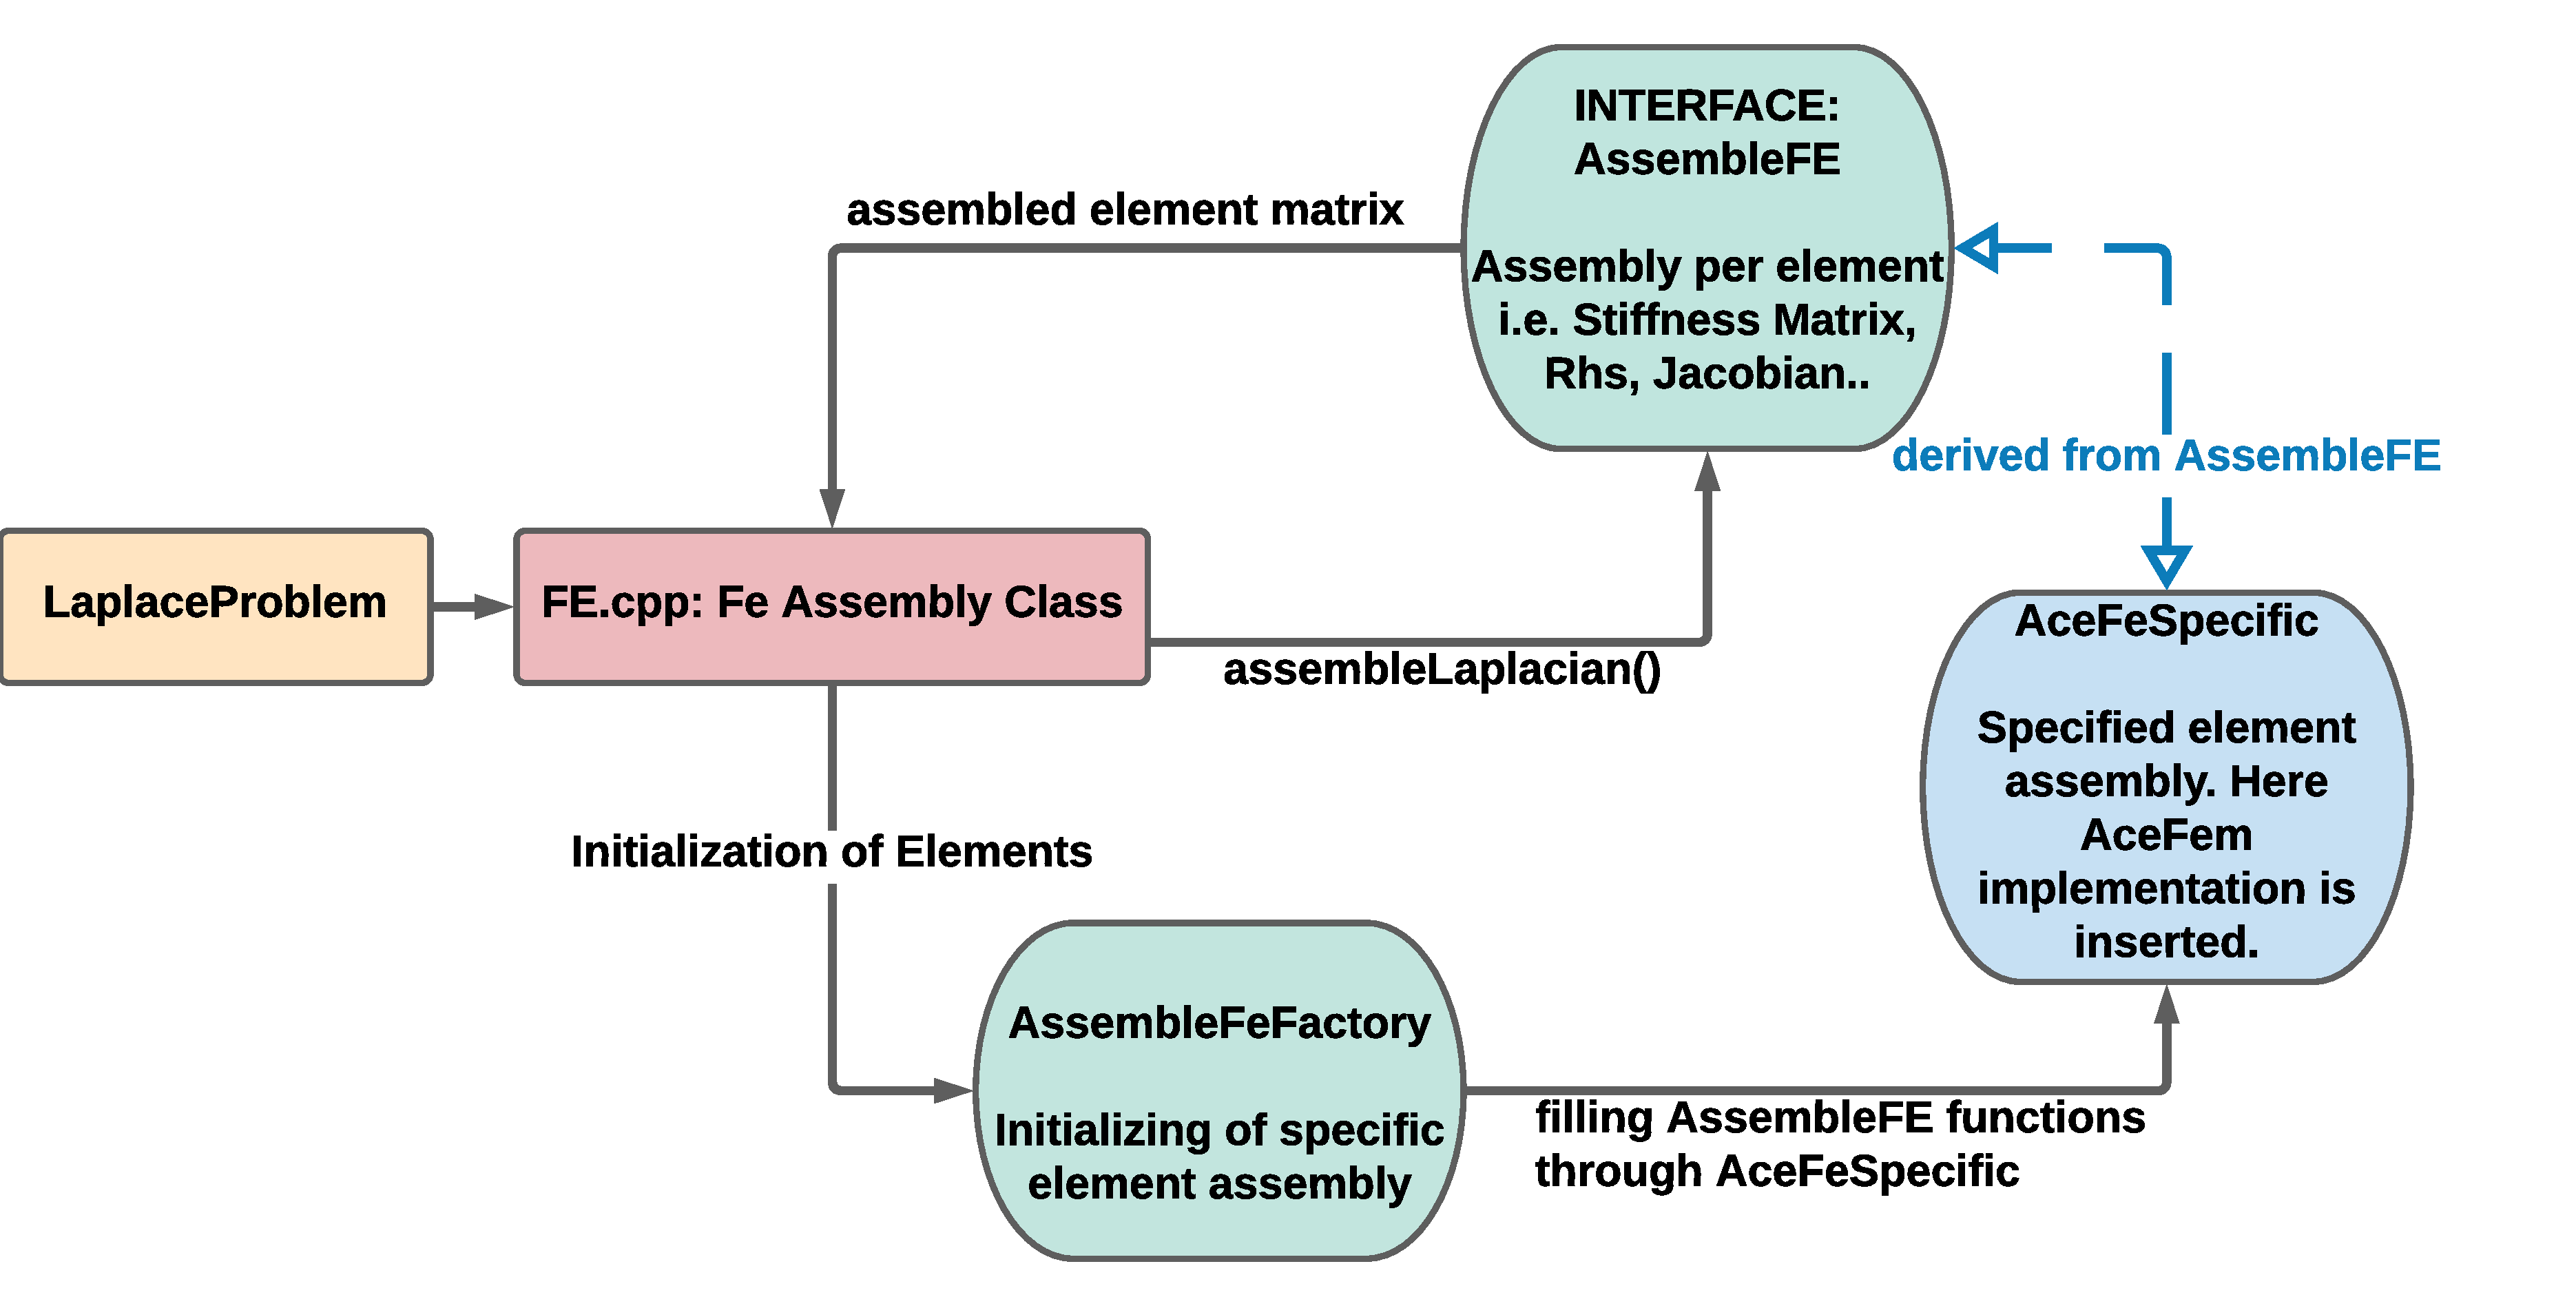
\includegraphics[width=1\textwidth , height=0.5\textwidth]{AceFe.pdf}
 \caption{Accessing AceFem Implementation. Example for assembling finite element stiffness matrix for Laplace problem.}
\end{figure}

For implementing the interface we need three new classes:
\begin{itemize}
\item \texttt{AssembleFE}
\item \texttt{AssembleFEFactory}
\item \texttt{AceFeSpecific}
\end{itemize}

\section{\texttt{AssembleFE} Class}
\texttt{AssembleFE} is the basis class and interface for the finite element assembly.\\
We access the \texttt{AssembleFE} Implementation in the general finite element assembling class \texttt{FE}.

$\rightarrow$ For each element we should be able to assemble different finite element entities, for example stiffness matrix, right hand side or Jacobian matrix, with the \texttt{AssembleFE} object.
\begin{lstlisting}
// Assembly of element matrix for laplacian operator
AssembleFE.assemblyLaplacian(); 
\end{lstlisting}
\captionof{lstlisting}{Calling \texttt{assemblyLaplacian()} of \texttt{AssembleFE} in \texttt{FE.cpp}}
~~\\
The \texttt{AssembleFE} class only owns virtual assembling functions.
\begin{lstlisting}
virtual void assemblyLaplacian() = 0;
virtual void assemblyRHS() = 0;
\end{lstlisting}
\captionof{lstlisting}{An example of virtual assembly functions of \texttt{AssembleFE}.}
~~\\
Those virtual functions are initialized through \texttt{AssembleFEFactory} with the corresponding \texttt{AceFeSpecific} assembly functions.

As an \texttt{AssembleFE} object represents one element, the implementation within \texttt{AssembleFE} is independent of any parallel implementation. The \texttt{FE} class distributes the local element matrices to the global matrices accordingly.

\section{\texttt{AssembleFEFactory} Class}
The \texttt{AssembleFEFactory} class fills the virtual functions of \texttt{AssembleFE} with the corresponding functions of the specific problem.
It builds the \texttt{AceFeSpecific} object of the \texttt{AssembleFE} basis object. 
\begin{lstlisting}
AssembleFEFactory(string problemType, AssembleFE_Type assembleFE ):
{
if(problemType == "Laplace"){
	assembleFE = new AceFeSpecificLaplace();
}
else if( ..)

}
\end{lstlisting}
\captionof{lstlisting}{Constructor of \texttt{AssembleFEFactory} that initializes the \texttt{assembleFE} object.}

\section{\texttt{AceFeSpecific} Class}

The \texttt{AceFeSpecific} class is derived from \texttt{AssembleFE} and extends the virtual functions with specific assembly rules.
Each specific problem corresponds to a \texttt{AceFeSpecific} class of functions. 

For a Laplace problem we would have a \texttt{AceFeSpecificLaplace} class with its corresponding assembly of right hand side and stiffness matrix (see Code \ref{CodeLaplace}).
 ~~\\
 
For adding a new element or assembly routine (or \textbf{AssembleFem} code), one must simply add a new or extend an \texttt{AceFeSpecific} class that fulfills \texttt{AssembleFE}'s assembly  requirements and add the build information to \texttt{AssembleFEFactory}. This way the element assembly can be accessed equally in the \texttt{FE} class for each specific assembly routine that is concealed in the \texttt{AceFeSpecific} classes. 
 ~~\\
 ~~\\
 ~~\\
\begin{lstlisting}
void assemblyLaplacian(Matrix &ElementMatrix){
	
    numNodes= nodesRefConfig_.size(); // number of nodes per element
    dPhi = this->getDPhi(dim_, FEType_); // nabla phi
    Matrix B(dim_); // transformation matrix
    Matrix Binv(dim_); // inverse of transformation matrix
    this->buildTransformation(B); // building inverse
    detB = B.computeInverse(Binv);  // determinent of inverse
    dPhiTrans = this->applyBTinv( dPhi,Binv ); // applying inverse to dPhi
    
    // Filling element matrix with correct values
    for (int i=0; i < numNodes; i++) {
        for (int j=0; j < numNodes; j++) {
            ElementMatrix[i][j] = //assembly rules; 
        }
    }
}
\end{lstlisting}
\captionof{lstlisting}{\texttt{AssemblyLaplacian()} in \texttt{AceFeSpecificLaplace}. }
\label{CodeLaplace}


%\newpage
%\section{Open Questions}
%\begin{itemize}
%\item How specific are the assembly functions?
%\item Where are basis functions, quadrature values and other useful functions stored (i.e. buildTransformation)?
%\item How exactly is the AceFeFactory build process of AceFeSpecific?
%\item What is the Output of assembly? Input\/Output Point or return value?
%\end{itemize}
%
%\chapter{Interface in Detail}
%
%\section{Basisclass}
%
%
%\textbf{The following functions are not uniquely defined for different problems and thus are not virtual functions, but implemented in \texttt{AceFe}}?
%\begin{lstlisting}[caption=Additional Functions and Features]
%updateSolution(); // i.e. for nonlinear iterations
%
%initParams(); // initializing important assembly params
%updateParams(); // updating parameters in case its needed
%
%advanceInTime(); // signaling advancement in time
%
%preProcessing(); //
%postProcessing(); //
%\end{lstlisting}
%
%Each \texttt{AceFe} element holds detailed information of the current problem.
%\begin{lstlisting}[caption=Variables]
%private:
%	string FEType_; // Finite Element discretization
%	int dim_; // Dimension
%	int dofs_; // Degrees of freedom
%	const int numNodes_; // Number of nodes (of element)
%	vec2D_dbl_Type nodesRefConfig_; // Nodes	
%	vec_dbl_Type paramsMaterial_; // Material Parameters
%	bool timeProblem_; // Time dependent problem
%	int flag_; // Element Flag
%	...
%\end{lstlisting}




~~~~ \\\

%\newpage

~~\\ 

%\bibliography{thesisbib}{}
%\bibliographystyle{plain}
%\addcontentsline{toc}{chapter}{Bibliography}


%\input{Erklaerung}






\end{document}
